\documentclass{article}
\usepackage{graphicx}
\usepackage{authblk}
\usepackage{amsmath}


\begin{document}
\title{THEORETICAL NEUROSCIENCE \\ EXERCISE 4}
\date{\today}
\author[1]{\c{S}eyma Bayrak\thanks{seyma.bayrak@st.ovgu.de}}
\affil[1]{\footnotesize  Otto von Guericke University of Magdeburg}
\maketitle

\section*{Introduction}

At each further exercise of Theoretical Neuroscience Course, we try a more realistic model for working mechanism of neuron. In exercise 3, the leaky integrate - fire (LIF) model of a neuron simulated already spike occurances due to imaginary action potentials. However, the time interval between spike occurances were always the same in LIF model. What happens in reality? The time intervals between subsequent spikes are not actually equal to each other, because of the opening-closing properties of ion channels. Exercise 4 aims to program spike occurances with varying spike rates with the so called \textit{"LIF model with spike frequency adaptation"}.\\

The LIF model with spike frequency adaptaion can be built step by step on Hodgkin-Huxlex Model, \textit{HHM}. A typical example of HHM can be stated as a single compartment model with one ion specific conductance ($K^{+}$) in addition to one leak conductane $g_{L}$ as given in equation 1.

\begin{equation}
 c_{m}\frac{dV_{m}(t)}{dt}=i_{e}-g_{K^{+}}(V-E_{K^{+}})-g_{L}(V-E_{L})
\end{equation}
The crucial poitn of this exercise to be able to express the conductance of potassium, $g_{K^{+}}$ as realistic as possible, since the adaptation of spike rate (or frequency) is designed as a $K^{+}$ conductance. $K^{+}$ conductance depends on the number of open $K^{+}$ channels on the cell membrane. The more depolarized the membrane potential is, $V_{m}$, the more the $K^{+}$ channels open. Therefore, $g_{K^{+}}$ increases with $V_{m}$ persistenlty in time.  The increase of $g_{K^{+}}$ is denoted by $\Delta g_{sra}$. The dynamic equations of SRA - spkie rate adaptation is given below. 

\begin{equation}
\tau_{sra}\frac{dg_{sra}}{dt}=-g_{sra} \,\,\,\,\,\,\,if\,\,\,\,\,\,\,V_{m}(t)<V_{th}
\end{equation}

\begin{equation}
 g_{sra}(t+dt)=g_{sra}+dg_{sra}\,\,\,\,\,\,\,if\,\,\,\,\,\,\,V_{th} \le V_{m}(t)
\end{equation}

The solution of equation 2 yields an exponential function as the following, $g_{sra}(t+dt)=g_{sra}(t).exp(-\frac{dt}{\tau_{sra}})$ while the Let us insert time dependent potassium ion conductance $g_{sra}(t)$ into equation 1 in order to get a dynamic equation for the membrane potential. 

\begin{equation}
 c_{m}\frac{dV_{m}(t)}{dt}=i_{e}-g_{L}(V_{m}(t)-E_{L})-g_{sra}(t)(V_{m}(t)-E_{K^{+}})
\end{equation}
It is to be reminded that, $g_{L}=\frac{1}{r_{m}}$ and $\tau_{m}=r_{m}.c_{m}$. The below math tricks are followed to get even more closely the dynamical equation for the $V_{m}$.


\begin{equation*}
c_{m}\frac{dV_{m}(t)}{dt}=i_{e}-V_{m}(t)(g_{L}+g_{sra}(t))+g_{L}E_{L}+g_{sra}E_{K}
\end{equation*}

\begin{equation*}
\frac{c_{m}}{g_{L}+g_{sra}(t)}\frac{dV_{m}(t)}{dt}=\frac{i_{e}+g_{L}E_{L}+g_{sra}E_{K}}{g_{L}+g_{sra}(t)}-V_{m}(t)
\end{equation*}

In order to make the dynamic equation seem simpler, such values as effective time constant $\tau_{eff}(t)$ and and effective equilibrium potential $V_{\infty}^{eff}(t)$ are defined as the following.

\begin{equation*}
 \tau_{eff}(t)=\frac{c_{m}}{g_{L}+g_{sra}(t)} \,\,\,\,\,\,\,\,\,\,\,V_{\infty}^{eff}(t)=\frac{i_{e}+g_{L}E_{L}+g_{rsa}E_{K}}{g_{L}+g_{sra}(t)}
\end{equation*}
Inserted fresh defined terms into equation 4 results in the simplest form of dynamic equation of $V_{m}$ as in equation 5. As it is realised, this is maybe only one step complicated version of the simple compartment model of $V_{m}$.

\begin{equation}
 \frac{dV_{m}(t)}{dt}=\frac{1}{\tau_{eff}(t)}[V_{\infty}^{eff}(t)-V_{m}(t)]
\end{equation}

The final step is to introduce the analytic solution of equation 5 in order to iterate it through time steps dt as shown below. The $V_{m}$ potential depends not only the time variable, but also commanded by the threshold potential, the same case for $g_{sra}$. 

\begin{equation}
 V_{t+dt}=V_{\infty}^{eff}(t)+[V_{m}(t)-V_{\infty}^{eff}(t)]exp(-\frac{dt}{\tau_{eff}}(t))\,\,\,\,\,if\,\,\,\,\,V_{m}(t+dt)<V_{th}
\end{equation}

\begin{equation}
 V_{m}(t+dt)=V_reset\,\,\,\,\,\,\,\,\,\,\,\,\,\,\,\,if\,\,\,\,\,\,\,\, V_{th} \le V_{m}(t+dt)
\end{equation}

\begin{center}
 \section*{Part 1}
\end{center}



The first part of programing assignment aims to plot two graphs: change in membrane potential by time, $V_{m}(t)$ vs $t$, and change in K+ channel conductivitiy by time, $g_{sra}(t)$ vs $t$. At the beginning, a time vector and a constant input current are defined.  The first computed value is $g_{sra}(t)$ as stated in equations 2 and 3. Second computation is done for $\tau_{eff}(t)$ and $V_{\infty}^{eff}(t)$. Now, all the parameters required for the iteration of $V_{m}(t)$ value are well defined, therefore the last step is to complete the derivation of $V_{m}(t)$ as in equations 6 and 7. Since the two limiting conditions for both $g_{sra}(t)$ and $V_{m}(t)$ are the same, which is the comparison of $V_{m}(t)$ with $V_{th}$, those two values can be easily calculated inside the same \textit{loop} under the same \textit{if statement}.\\

The parameters are defined just before starting the \textit{loop} at programing-editor as the following.\\

$
T=600 ms\,\,\,\,\,\,\ dt=0.1 ms\,\,\,\,\,\,\ i_{e}=12 nA/mm^2 \,\,\,\,\,\,\ c_{m}=15 nF/mm^2 $


$
E_{L}=V_reset=-65 mV\,\,\,\,\,\,\ E_{K^{+}=-75 mV}\,\,\,\,\,\,\ V_{th}=-45 mV\,\,\,\,\,\,\ V_{m}(t=0)=E_{L} $

$
g_{L}=0.5 \mu S/mm^{2}\,\,\,\,\,\,\ dg_{sra}=0.05 \mu S/mm^{2}\,\,\,\,\,\,\ g_{sra}(t=0)=0 \mu S/mm^2 \,\,\,\,\,\,\  $

$ \tau_{sra}=250 ms $ \\

The following graph is plotted successfully.\\

\begin{center}
 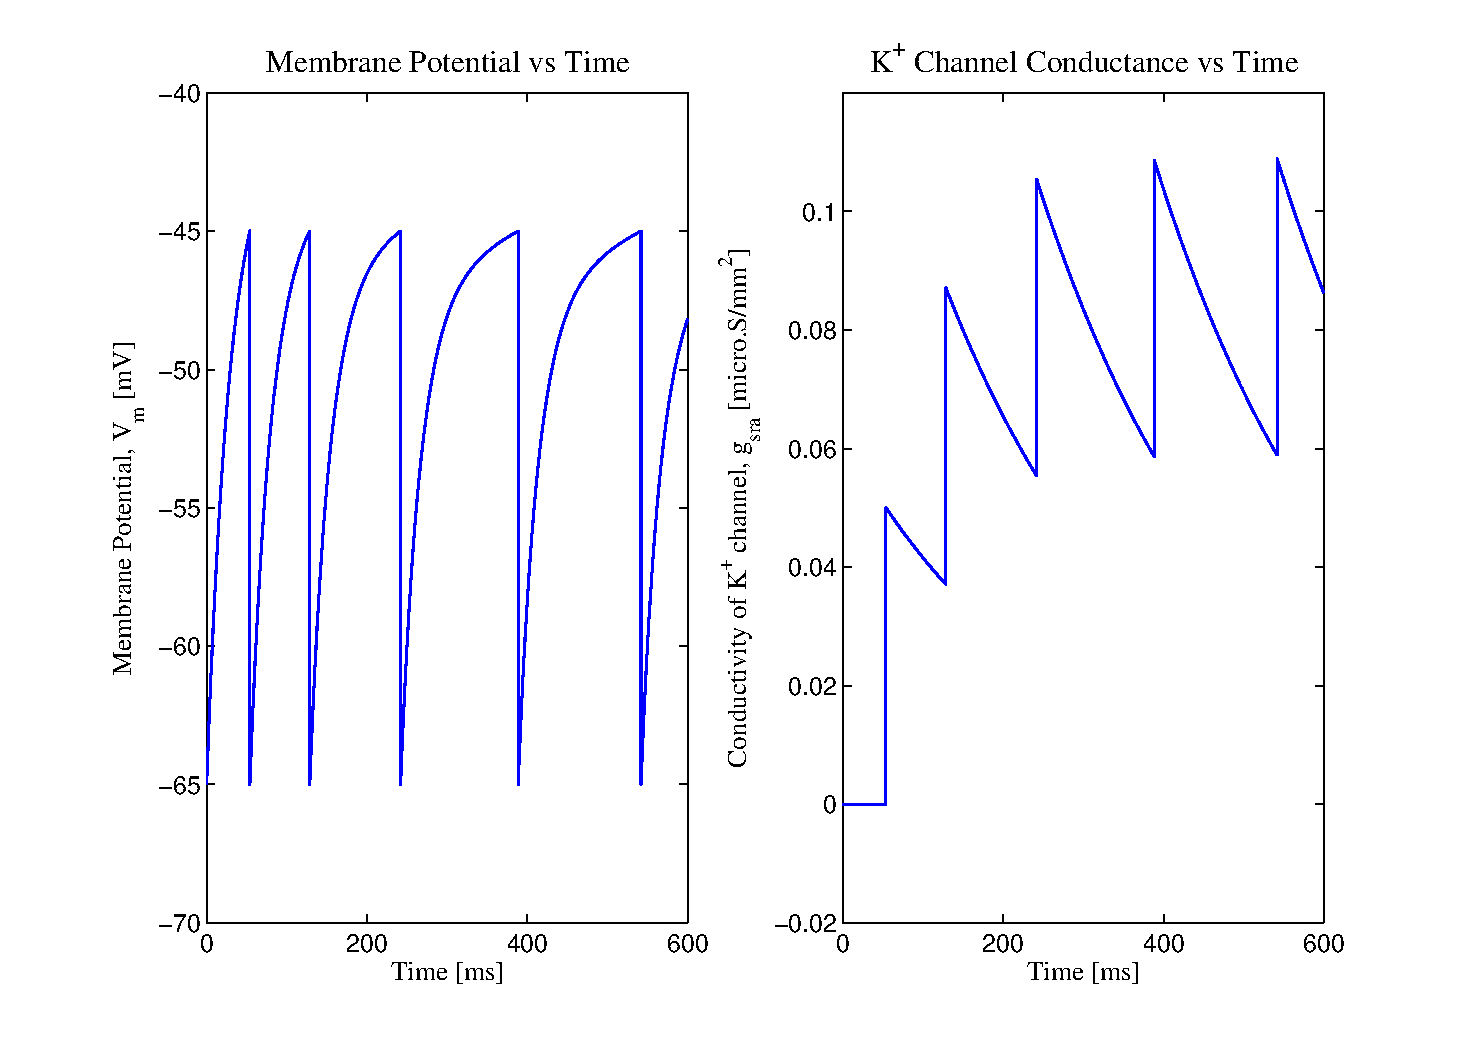
\includegraphics[width=\textwidth]{fig1.eps}
 % q7.eps: 0x0 pixel, 300dpi, 0.00x0.00 cm, bb=  -86   231   682   610
\begin{footnotesize}Graph 1, The graph on the left side indicates what happens to membrane potential as it reaches to the threshold value under varying time. The graph on the right side shows the change in conductivity of potassium channel in time.\end{footnotesize}
\end{center}

\begin{center}
\section*{Part 2} 
\end{center}

The second part of programming exercise is to create a \textit{function} on MATLAB, which calculates the spike rate at any given value of $dg_{sra}$, which is the iterative change among sequent $g_{sra}$ values. \\

At the first part, a model for the $V_{m}$ is already simulated. We are now interested in "when and how often spikes occur". Whenever a spkie on $V_{m}$ is observed, the corresponding time point is saved, then the time interval between any interested two spikes can be easily found. In this exercise, the time interval $t_{isi}$ between last two spikes at $V_{m}$ is calculated. Now, the key step of Part 2 is to find the spkie rate $r_{isi}$ just by the formula $1/t_{isi}.$ \\

The programmed function is named as \textit{sra\_LIF}, this function gets the input value for $dg_{sra}$, and then creates proper $V_{m}$, $g_{sra}$, $t_{isi}$ values,  and at the end displays the output as $r_{isi}$ - spkie rate at the command window. The table below is printed out by using sra\_LIF function for different input values. \\

\begin {table} [h]
 \begin{center}
  \begin{tabular}{ l | c | r }

    
$dg_{sra}$ & $r_{isi}$ \\
$(\mu S/mm^{2})$ & $(Hz)$
 \\ \hline \hline
 
    0.00 & 18.55 \\ \hline
    0.03 & 09.14 \\ \hline
    0.05 & 06.51 \\ \hline
    0.07 & 05.14 \\ \hline
    0.09 & 04.35 \\ \hline
    0.12 & 03.63 \\ \hline
    0.15 & 03.18 \\ \hline

  \end{tabular}

 
\begin{footnotesize} 
$ $\\ Table 1  
 \end{footnotesize}

\end{center}
\end{table}



\begin{center}
\section*{Part 3} 
\end{center}

The last part of exercise aims to simulate the change in spike rate under changing values of $dg_{sra}$. It sounds very similar to the Part 2, but this time, instead of calling output value of sra\_LIF function on command window for each different input value, it is computed aoutomatically in another \textit{Editor} of MATLAB. At the end, the graph of $dg_{sra}$ versus spike rate, or in other words, spike frequency is plotted. \\

A vector for different values of $dg_{sra}$ is created, it varies from the value of $0$ $\mu S/mm^2$ in steps of $0.05$ $\mu S/mm^2$  up to $0.15$ $\mu S/mm^2$. How to calculate $r_{isi}$ for varying $dg_{sra}$ values as easy as possible without calling the function  on command window? The answer is to use sra\_LIF function inside a \textit{loop} for each different $dg_{sra}$ and save the output $r_{isi}$ in another vector. The very last step of programing part is just to plot input values $dg_{sra}$ versus output values $r_{isi}$, as given by graph 2.

\begin{center}
 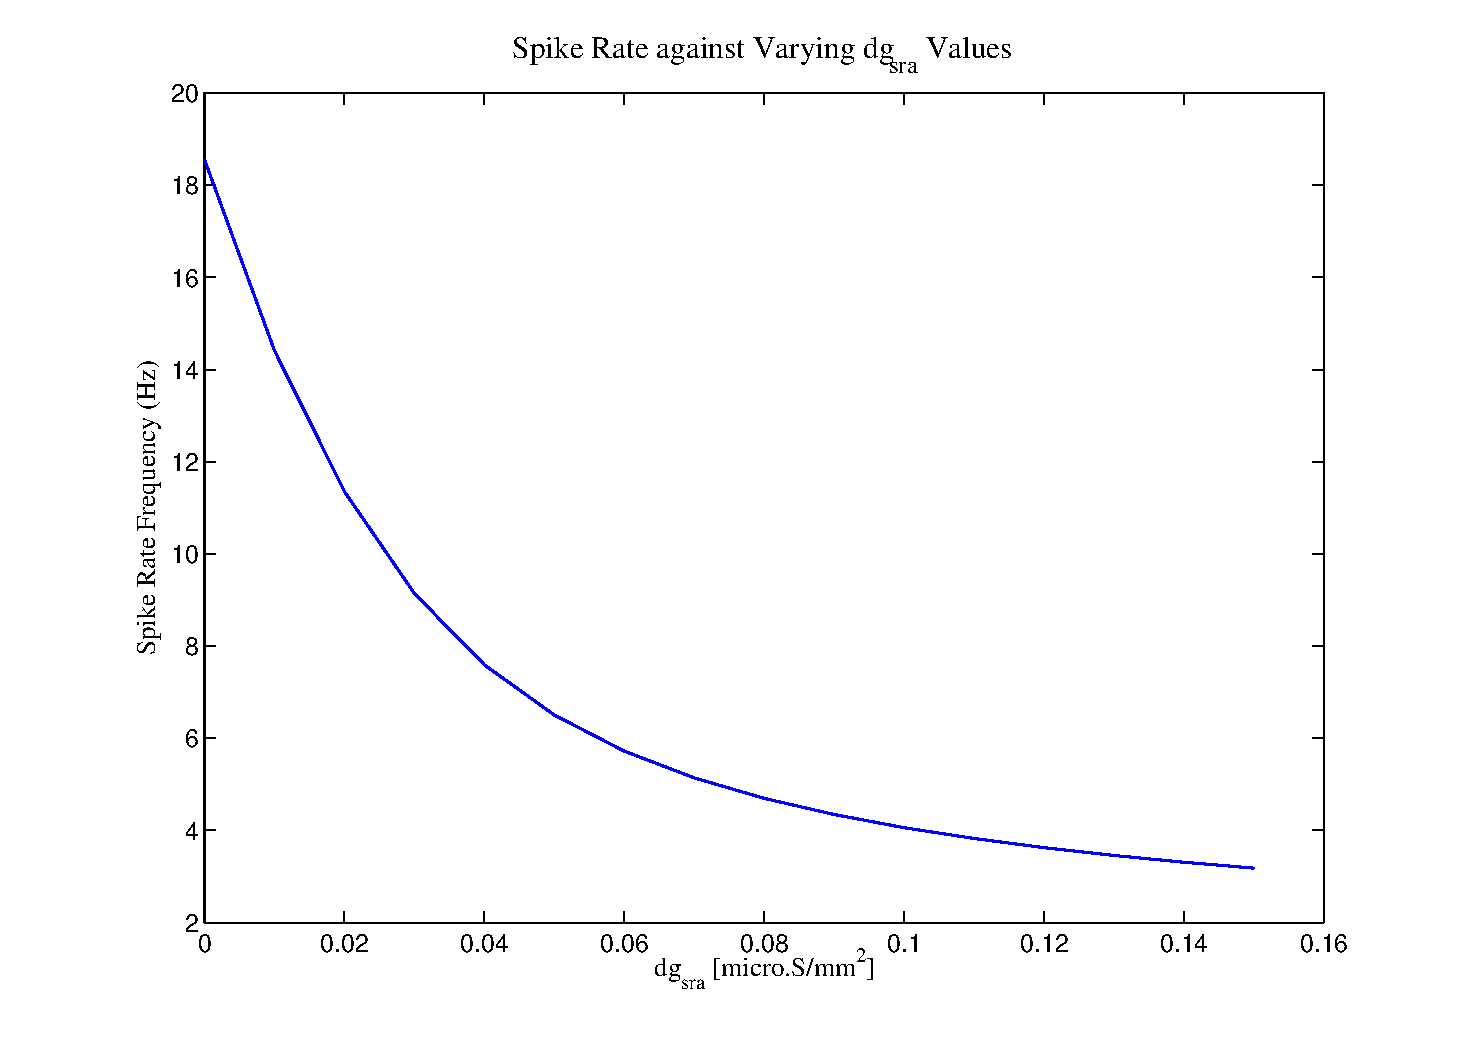
\includegraphics[width=\textwidth]{fig2.eps}
 % q7.eps: 0x0 pixel, 300dpi, 0.00x0.00 cm, bb=  -86   231   682   610
\begin{footnotesize}Graph 2, For each different value of $dg_{sra}$, the sra\_LIF function computes the corresponting spike frequency. At the end the two vectors of input and output is to be plotted. \end{footnotesize}
\end{center}


\section*{Discussion} 

In the LIF model without spike rate adaptation (SRA), it was previously observed that, the spikes of $V_{m}$ occurs just after following same time intervals. However, in the LIF model with SRA, the time interval between spikes get longer as seen on Graph 1. The simulations from Part 1 also shows that, the conductance of $K^{+}$ channels, is inreased by spikes.\\

Since $E_{K}=-70 mV$, the opening of $K^{+}$ channels counteracts the membrane potential polarization. Potassium wants $V_{m}$ to be close to $E_{K}$! It sounds complicated but maybe summarized as the following: Depolarization of $V_{m}$ inreases $g_{sra}$, but this increment hyperpolarize the neuron (because $E_{k}<V_{m}$ ), and reduce the spike frequency.\\

 Part 2 and 3 indicate that, the greater the iterative change in $g_{sra}$, so called $dg_{sra}$, the less the spike frequency is. When the conductance is inreased by greater amounts of $dg_{sra}$, the spike frequencyrelaxes exponentially to zero with time constant $\tau_{sra}$ as equation 2 states. 


\end{document}
